\chapter{Introduction}
\label{chap:intro}

\section{Proof Assistants}

Proof assistants, also known as interactive theorem provers (ITPs),
are software tools used in mathematics, computer science, and formal methods
to assist in the development and verification of mathematical proofs.
These tools play a crucial role in ensuring the correctness and reliability
of complex mathematical statements and software systems.
Examples of such tools include Agda~\cite{BoveDybjerNorell2009}, Coq~\cite{BertotCasteran2013}, and Lean~\cite{deMouraUllrich2021}.

Although similar in principal to typechecking in programming languages,
proof checking is normally seen as an interactive process between the mathematician and a proof assistant.
To this end, most proof assistants provide some interactive features either through specialized IDEs
(e.g. CoqIDE\footnote{\url{https://coq.inria.fr/refman/practical-tools/coqide.html}}),
integrating via Proof General~\cite{Aspinall2000}, or Visual Studio Code
(via the Language Server Protocol (LSP)~\cite{Gunasinghe2022}).
Most well-established proof assistants support several of these options.

\Rzk{}~\cite{Kudasov2023-github-rzk} is a new proof assistant that is based on Riehl-Shulman's type theory for synthetic $\infty$-categories~\cite{RiehlShulman2017, Riehl2023}.
The proof assistant is experimental but has been successfully used recently to formalize some fundamental results for $\infty$-categories,
including the $\infty$-categorical Yoneda lemma~\cite{Kudasov2023}.
However, \Rzk{} lacked most of the aforementioned features that are usually found in theorem provers, such as interactivity and syntax highlighting.
This paper reports on the implementation of utility and interactive tools around \Rzk{} proof assistant, focusing on the language server and VS Code extension support.
The goal is to provide a more user-friendly interface for \Rzk{} that would make it easier to use for both beginners and experienced users.

\section{Language Servers}

A few years ago, when a new code editor was introduced,
it needed to support the most popular programming languages,
and depended on plugins written specifically for this editor to support languages not built into the editor.
This led to a lot of repetitive work to provide useful language feature for the same language on multiple editors,
and an inconsistency between the provided language features on different editors.
The idea of language servers is Microsoft's attempt to solve this problem by standardizing a protocol for communication between a code editor (the client) and a background process (the server) that provides the language features for a certain language. This protocol is known as Language Server Protocol (LSP) \cite{Gunasinghe2022}. With LSP, a language author need only implement the server once and would automatically get language support on any editor that supports LSP. Likewise, an editor that supports LSP would automatically get language support for any programming language that has an LSP server. Examples for the language features in question include providing diagnostic messages, jumping to the location an identifier is introduced, text completion, semantic syntax highlighting, and much more.

\begin{figure}
  \centering
  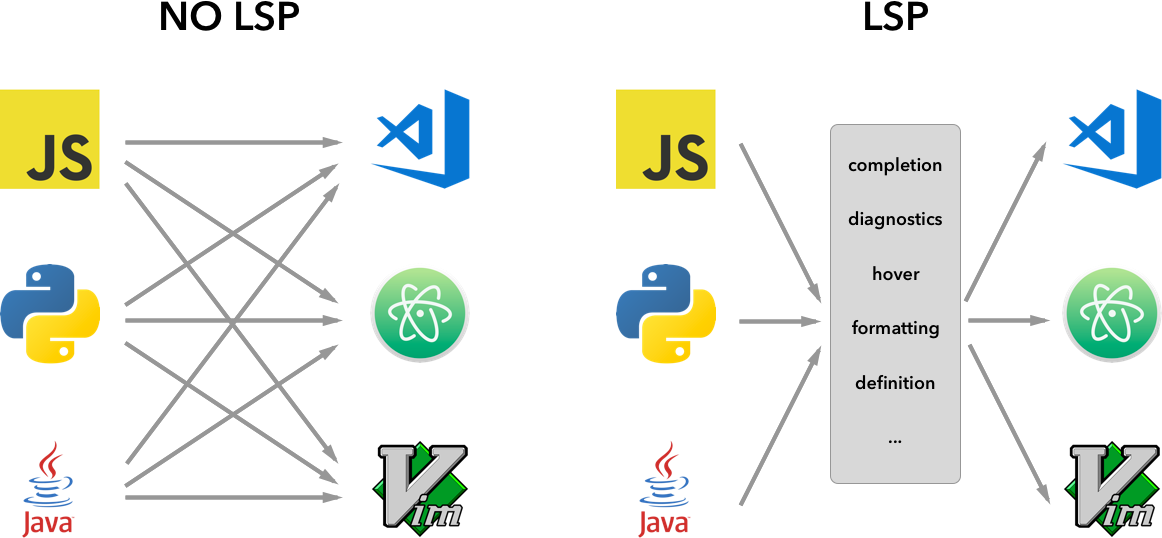
\includegraphics[width=0.7\textwidth]{figs/LSP-MxN.png}
  \label{figure:lsp}
  \caption{
    The motivation behind LSP, from Microsoft's website.
    \protect\footnotemark
  }
\end{figure}
\footnotetext{\raggedright\url{https://code.visualstudio.com/api/language-extensions/language-server-extension-guide}}

This protocol is particularly useful for interactive theorem provers since
they rely on the editing experience much more than a command line interface.
This is due to the fact that theorem provers generally do not need to compile
to any kind of executable file and only need the type-checking stage of compilers,
which can be easily performed by a language server. However, this also adds extra work
on the language server since it needs to support more features than a regular compiler would,
including listing variables in context along with their types, supporting Unicode symbols,
and most importantly allowing for an interactive step-by-step proof walkthrough.

\section{Contribution}

In this paper, we report on the work-in-progress on the implementation of
utility and interactive tools around \Rzk{} proof assistant, focusing on
the language server and VS Code extension support.
An earlier report on the progress of this work was also presented at the PSSV 2023
\cite{PSSV2023} conference in Innopolis University.

The contributions reported on include the following:
\begin{itemize}
  \item A language server for \Rzk{} that supports basic LSP features such as diagnostics, code completions, and semantic highlighitng.
  \item A VS Code extension that allows users to easily download and use the language server.
  \item A code formatter for \Rzk{} code.
  \item A plugin for MkDocs that allows for rendering \Rzk{} code snippets in Markdown documents.
  \item Integrating the previously mentioned additions to existing \Rzk{} formalization projects.
\end{itemize}
